\documentclass[aspectratio=169]{beamer}
\usepackage{appendixnumberbeamer}
\usetheme{metropolis}           % Use metropolis theme
\definecolor{fhggreen}{RGB}{23,156,125}
\let\oldemph\textbf
\renewcommand{\textbf}[1]{{\color{mLightBrown}\oldemph{#1}}}

\usepackage{blkarray}
\usepackage{amsmath}
\usepackage{multirow}
\title{The $R^5N$ Distributed Hash Table\\\small{IETF118}}
\date{06/11/2023}
\author{\textbf{Martin Schanzenbach~$\spadesuit$}, Christian Grothoff~$\clubsuit$, Bernd Fix~$\diamondsuit$}
%\institute{\hfill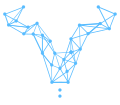
\includegraphics[trim={0cm 1.5cm 0cm 0cm},clip,width=6em]{gnunet}\url{https://gnunet.org}}
\institute{$\spadesuit$~Fraunhofer AISEC \url{https://aisec.fraunhofer.de}\\$\clubsuit$~Berner Fachhochschule \url{https://bfh.ch}\\$\diamondsuit$~GNUnet e.V. \url{https://gnunet.org}}
\begin{document}
  \metroset{block=fill,sectionpage=progressbar,numbering=counter}
  \maketitle

% \section{The R5N DHT In a Nutshell}

\begin{frame}{$R^5N$: Randomized-recursive routing for restricted-route networks}
  $R^5N$ is a DHT with the following design goals:
  \begin{itemize}
    \item \textbf{Open participation peer-to-peer routing}.
    \item Works in \textbf{restricted-route environments}.
    \item Supports \textbf{route path recording}.
    \item In-band \textbf{request (and response) validation}.
    \item Allows for \textbf{result filtering}.
  \end{itemize}
  I-D: \url{https://datatracker.ietf.org/doc/draft-schanzen-r5n/}
\end{frame}

\begin{frame}{Open participation peer-to-peer routing}
  \begin{itemize}
    \item Access control requires authentication (and trust) and leads to centralization.
    \item RELOAD (RFC 6940): ``\textit{RELOAD's security model is based on each node having one or more
   public key certificates.  In general, these certificates will be
   assigned by a central server, which also assigns Node-IDs, although
      self-signed certificates can be used in closed networks.}''
    \item (Popular) DHTs today require classic Kademlia-style ad-hoc permissionless participation (e.g. IPFS).
  \end{itemize}
\end{frame}


\begin{frame}{Support for restricted-route environments}
  From ``$R^5N$ : Randomized Recursive Routing for
Restricted-Route Networks'' by Evans et al.:
  \begin{itemize}
    \item \textit{Restricted-route topology} refers to a connected underlay topology which does not support direct
      connections between some of the nodes (e.g. wireless mesh networks, NAT or firewalls).
    \item Common DHT routing algorithms (e.g. Kademlia) show diminished performance or even arrant failure when operating over a restricted-route underlay.
    \item A common solution is to prevent participation in the DHT to peers that are not encumbered by such restrictions.
    \item However, on the modern Internet the proportion of hosts with unrestricted communication capabilities is increasingly limited (e.g. CG NAT).
  \end{itemize}
\end{frame}

\begin{frame}{Implications of restricted-route environments}
  Problem:
  \begin{itemize}
    \item Some peers, which from the distance metric (XOR) may be close, may not be reachable (e.g. firewall).
    \item This leads to multiple (local) minima with respect to where data may be stored/can be retrieved.
  \end{itemize}
  Solution:
      \begin{itemize}
        \item Random walk before greedy decent to ``escape'' local minima.
        \item Assuming we have a small world topology, the random walk will cause us to land at a random peer in the network from where the greedy descent will find a random local minimum.
        \item Replication at multiple local minima combined with the birthday paradox provides reasonable availability.
      \end{itemize}
\end{frame}

\begin{frame}{Kademlia sunshine scenario (k=2)}
  \begin{center}
    \includegraphics[height=0.9\textheight]{R5NRoutExample-0.pdf}
  \end{center}
\end{frame}

\begin{frame}{Restricted route scenario}
  \begin{center}
    \includegraphics[height=0.9\textheight]{R5NRoutExample-1.pdf}
  \end{center}
\end{frame}
\begin{frame}{Local minima I}
  \begin{center}
    \includegraphics[height=0.9\textheight]{R5NRoutExample-2.pdf}
  \end{center}
\end{frame}

\begin{frame}{Local minima II}
  \begin{center}
    \includegraphics[height=0.9\textheight]{R5NRoutExample-3.pdf}
  \end{center}
\end{frame}

\begin{frame}{PUT example --- XOR}
  \begin{center}
    \includegraphics[height=0.9\textheight]{R5NRoutExample-5.pdf}
  \end{center}
\end{frame}

\begin{frame}{PUT example --- $R^5N$ walk length $= 1$}
  \begin{center}
    \includegraphics[height=0.9\textheight]{R5NRoutExample-6.pdf}
  \end{center}
\end{frame}

\begin{frame}{PUT example --- $R^5N$ walk length $= 1$}
  \begin{center}
    \includegraphics[height=0.9\textheight]{R5NRoutExample-7.pdf}
  \end{center}
\end{frame}

\begin{frame}{Special case: At least one descent-hop; no loops}
  \begin{center}
    \includegraphics[height=0.9\textheight]{R5NRoutExample-8.pdf}
  \end{center}
\end{frame}

\begin{frame}{Route recording for source routing}
  Consider the following problem:
  \begin{itemize}
    \item Two peers want to use a communication channel.
    \item They cannot establish a direct link due to underlay restrictions.
    \item Assumption: Other peers are happy to provide relay services.
    \item Payload transmission via PUT and GET would be inefficient.
  \end{itemize}
  $\Rightarrow$ Discover a route through the overlay:

  \begin{itemize}
    \item Peer adverstises existence of service via DHT PUT with route recording.
    \item Client discovers service provider via DHT GET with valid route of GET/PUT message path.
  \end{itemize}
\end{frame}


\begin{frame}{In-band response validation}
  DHT values can be corrupted or invalid. $R^5N$ addresses this with pluggable, extensible block types:
  \begin{itemize}
    \item Given a key and a block type, it is possible to verify the integrity of the value.
    \item The verification should be possible for all hops on path, improving caching performance.
    \item A verification could include cryptographic signatures over the data or more sophisticated approaches (see GNS, RFC-to-be 9498)
  \end{itemize}
\end{frame}

\begin{frame}{Result filtering via mutated Bloom filter}
  Queries could have a unique or multiple results depending on the application.
  \begin{itemize}
    \item We provide capability to abort query forwarding early if unique answer has been found.
    \item We probalistically filter results already known to the client to reduce traffic.
    \item To address false positives when using Bloom filters we use mutation.
  \end{itemize}
\end{frame}

\begin{frame}{Optimization: Routing loop prevention}
  Repeatedly visiting the same peer in GET or PUT operations is inefficient.
  \begin{itemize}
    \item Visiting new peers increases the chance of finding previously undiscovered results.
    \item Visiting new peers drives us away from the starting point and towards more distant local minima.
  \end{itemize}
  $R^5N$ uses a \textit{Bloom filter} in GET/PUT messages to prevent routing loops.
\end{frame}

\begin{frame}{For DISPATCH}
  \begin{itemize}
    \item I-D is WIP at \url{https://datatracker.ietf.org/doc/draft-schanzen-r5n/}\\
    \item We have approached WGs since initial upload: dinrg, rtgwg, \ldots
    \item Which (other) WGs may be interested?
  \end{itemize}
\end{frame}

\begin{frame}
  \begin{center}
    \centering Funded by\\
    
\includegraphics[width=2cm]{ngi.png}\qquad
\includegraphics[width=2cm]{nlnet.png}
    %\vspace{1cm}\\
    %DISPATCH: Are there any WGs interested in adopting/working on this?\\
    \vspace{2em}
    \\Contacts:\\
    \vspace{1em}
    {\tiny
    Martin Schanzenbach \texttt{schanzen@gnunet.org}\\
    Christian Grothoff \texttt{grothoff@gnunet.org}
    }
  \end{center}
\end{frame}

\appendix

\end{document}
